% =========================================================================== %
% Preamble                                                                    %
% =========================================================================== %

\documentclass[12pt, dvipsnames, aspectratio=169]{beamer}
%\documentclass[12pt, dipsnames, notes=only]{beamer}

\usepackage[utf8]{inputenc}
\usepackage{beamerthemesimple}

\date{February 24$^{th}$, 2021}
\title{Spectre Attacks}
\author{William Findlay}
\institute{Carleton University\\\href{mailto:will@ccsl.carleton.ca}{\ttfamily will@ccsl.carleton.ca}}

\usepackage{csquotes}
\usepackage{booktabs}

% Center floats by default
\makeatletter
\g@addto@macro\@floatboxreset{\centering}
\makeatother

\usepackage{listings}

\lstnewenvironment{listing}[1][]{\lstset{#1}}{}

\definecolor[named]{red}{HTML}{A4031F}
\definecolor[named]{blue}{HTML}{0071B2}
\definecolor[named]{orange}{HTML}{E59C00}
\definecolor[named]{green}{HTML}{009E73}
\definecolor[named]{purple}{HTML}{88498F}
\definecolor[named]{dark-grey}{HTML}{515151}
\definecolor[named]{grey}{HTML}{797979}

\colorlet{listing-basic}{dark-grey}
\colorlet{listing-keyword}{blue}
\colorlet{listing-keyword-2}{orange}
\colorlet{listing-keyword-3}{purple}
\colorlet{listing-comment}{grey}
\colorlet{listing-string}{green}

% Set default listings style
\lstdefinestyle{listingstyle}{
    basicstyle       = {\ttfamily\color{listing-basic}\lst@ifdisplaystyle\scriptsize\fi},
    keywordstyle     = {\color{listing-keyword}\bfseries},
    keywordstyle     = {[2]\color{listing-keyword-2}\bfseries},
    keywordstyle     = {[3]\color{listing-keyword-3}\bfseries},
    identifierstyle  = {\color{listing-keyword-3}\bfseries},
    sensitive        = true,
    commentstyle     = {\color{listing-comment}},
    stringstyle      = {\color{listing-string}},
    showstringspaces = false,
    columns          = fullflexible,
    keepspaces       = true,
    literate         = {~}{$\sim$}{1},
    escapeinside     = {!@}{@!}
}
\lstset{style=listingstyle}

% x64 asm language
\lstdefinelanguage
   {x64}     % add a "x64" dialect of Assembler
   [x86masm]{Assembler} % based on the "x86masm" dialect
   % with these extra keywords:
   {morekeywords={cdqe,cqo,cmpsq,cmpxchg16b,jrcxz,lodsq,movsxd, %
                  popfq,pushfq,scasq,stosq,iretq,rdtscp,swapgs, %
                  leaq,movq,movl,pause,lfence, %
                  rax,rdx,rcx,rbx,rsi,rdi,rsp,rbp,rip, %
                  r8,r8d,r8w,r8b,r9,r9d,r9w,r9b, %
                  r10,r10d,r10w,r10b,r11,r11d,r11w,r11b, %
                  r12,r12d,r12w,r12b,r13,r13d,r13w,r13b, %
                  r14,r14d,r14w,r14b,r15,r15d,r15w,r15b}} % etc.

% Define "none" language for listings
\lstdefinelanguage{none}{
  identifierstyle = {\color{listing-basic}}
}

\setbeamertemplate{section in toc}[sections numbered]

\hypersetup{
    colorlinks = true,
    linkcolor  = .,
    urlcolor   = blue,
    citecolor  = blue,
}
\urlstyle{tt}

\newcommand{\fullframegraphic}[1]{%
    {%
        \setwatermark{}
        \usebackgroundtemplate{\includegraphics[width=\paperwidth]{#1}}
        \begin{frame}[plain]
        \end{frame}
    }
}

\newcommand\ufootnote[1]{%
    \begingroup
        \renewcommand\thefootnote{}\footnote{\hspace{-1.8em}#1}%
        \addtocounter{footnote}{-1}%
    \endgroup
}

% Table of Contents for sections
\AtBeginSection[]
{
    \setwatermark{}
    \begin{frame}[c, noframenumbering, plain]
        \begin{center}
        \fontsize{36}{42} \selectfont \bfseries \color{destacado} \insertsection%
        \end{center}
    \end{frame}
}

\usepackage{biblatex}
\bibliography{refs.bib}
\renewcommand*{\bibfont}{\footnotesize}

\PassOptionsToPackage{hyphens}{url}
%\setcounter{biburllcpenalty}{1}
%\setcounter{biburlucpenalty}{1}
%\setcounter{biburlbigbreakpenalty}{2}
%\setcounter{biburlbreakpenalty}{1}

\usepackage{appendixnumberbeamer}

\makeatletter
\g@addto@macro{\UrlNoBreaks}{\do:}
\g@addto@macro{\UrlBreaks}{\do/}
\makeatother

\newenvironment{nscenter}
 {\parskip=0pt\par\nopagebreak\centering}
 {\par\noindent\ignorespacesafterend}

\let\lsi\lstinline%
\newcommand{\code}[1]{\lsi[language=c]|#1|}

\usepackage{svg}
\usepackage{mathtools}
\usepackage[normalem]{ulem}

\newcommand{\todo}[1]{{\color{orange}[#1]}}

\newcommand{\red}[1]{{\color{red}#1}}
\newcommand{\orange}[1]{{\color{orange}#1}}
\newcommand{\blue}[1]{{\color{blue}#1}}
\newcommand{\purple}[1]{{\color{purple}#1}}
\newcommand{\green}[1]{{\color{green}#1}}

% =========================================================================== %
% Document                                                                    %
% =========================================================================== %

\begin{document}

% Optional watermark
\setwatermark[hoffset=0.3cm, voffset=0.3cm]{
\includegraphics[width=8cm]{figs/logos/griffin.png}}

% Title page
\begin{frame}[noframenumbering, plain]
  \titlepage%
  \vfill
  \vspace{4em}
  {\footnotesize COMP5900X Discussion Lead}
\end{frame}

%\begin{frame}[c, noframenumbering, plain]{Outline of this Talk}
%    \tableofcontents
%\end{frame}
%
%\section{Untitled Section}

\begin{frame}[c]{Paper Overview}{}
  {\bf Title}
  \begin{itemize}
    \item \enquote{GRIFFIN: Guarding Control Flows Using Intel Processor Trace}
  \end{itemize}

  \vfill
  {\bf Authors}
  \begin{itemize}
    \item Xinyang Ge, Weidong Cui, Trent Jaeger
    \item Microsoft Research, Pennsylvania State University
    \item You might know Trent Jaeger from his excellent OS security textbook~\todo{CITE}
  \end{itemize}

  \vfill
  {\bf Venue}
  \begin{itemize}
    \item ASPLOS 2017
    \item Architectural Support for Programming Languages and Operating Systems
    \item Recognized as a flagship conference in hardware / OS design
    %\item Not really a security venue per se
  \end{itemize}
\end{frame}

\begin{frame}[c]{Goals}{}
  {\bf Problem Statement}
  \begin{itemize}
    \item Defenders can use CFI defences to mitigate code reuse attacks
    \item Most existing CFI defences are software-only
    \begin{itemize}
      \item Slow, inflexible, or incomplete protection
    \end{itemize}
    \item Hardware-backed CFI can offer better performance, security, flexibility
  \end{itemize}

  \vfill
  {\bf Claims / Contributions}
  \begin{itemize}
    \item Griffin $\rightarrow$ first online CFI implementation backed by Intel PT hardware
    \item Multiple policy granularities for flexibility (performance vs security at runtime)
    \item Performance is comparable to software-only CFI, but with better security
    \item Present possible optimizations for further performance improvements
  \end{itemize}
\end{frame}

\begin{frame}[c]{Threat Model and Assumptions}{}
  {\bf \color{blue} Trusted}
  \begin{itemize}
    \item The protected programs themselves (assumed benign)
    \begin{itemize}
      \item But they might contain logic errors / memory corruption vulnerabilities
    \end{itemize}
    \item The operating system (including \blue{all ring 0 code})
    \begin{itemize}
      \item Otherwise attacker could subvert / disable / bypass Griffin
    \end{itemize}
  \end{itemize}

  \vfill
  {\bf \color{orange} Not Trusted}
  \begin{itemize}
    \item Input into protected applications
    \begin{itemize}
      \item Could be used for \orange{memory corruption attacks}
    \end{itemize}
  \end{itemize}

  \vfill
  {\bf \color{green} Assumptions}
  \begin{itemize}
    \item Protected applications implement $W\oplus X$ defence
    \begin{itemize}
      \item Application cannot modify its own code
      \item Application cannot map pages as both writable and executable
    \end{itemize}
  \end{itemize}
\end{frame}

\section{Background}

\begin{frame}[c]{Memory Corruption / Code Reuse Attacks}{}
\begin{center}
  \color{black}%
  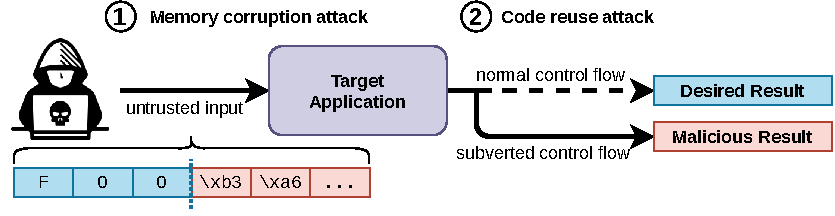
\includegraphics[width=0.8\columnwidth]{figs/memory_corruption.pdf}
\end{center}

\vfill
\begin{itemize}
  \item Memory corruption attack (e.g.~buffer overflow, use-after-free)
  \item Code reuse attack (e.g.~ROP, JOP, ret2libc)
  \item The point is to achieve some attacker goal by subverting normal control flow
  \begin{itemize}
    \item Spawn a shell, write to a sensitive file, etc.
  \end{itemize}
\end{itemize}
\end{frame}

\begin{frame}[c]{Control Flow Integrity: Overview}{}
{\bf The Basic Idea}
\begin{itemize}
  \item Identify correct code paths for an application $\rightarrow$ control flow graph (CFG)
  \item Enforce correct code paths at runtime (i.e.~they must follow the CFG)
  \item Control flow integrity can stop (most) code reuse attacks
  \begin{itemize}
    \item Depends on sophistication of the attack, granularity of CFI policy
    \item It at least significantly raises the bar for attackers
  \end{itemize}
\end{itemize}

\vfill
{\bf Software CFI Categories}
\begin{enumerate}
  \item Compile-time instrumentation
  \item Static binary instrumentation
  \item Runtime instrumentation
\end{enumerate}
\end{frame}

% FIXME/TODO: Verify the following three slides for accuracy

\begin{frame}[c]{Compile-Time Instrumentation}{}
  \begin{itemize}
    \item Extend compiler to generate correct CFG for compiled programs
    \item Enforce CFI in language runtime (here, runtime $\equiv$ code you did not write)
  \end{itemize}

  \vfill
  {\bf \blue{Benefits}}
  \begin{itemize}
    \item More efficient than other methods
    \item Easy to capture stateful control flow in CFG model
  \end{itemize}

  \vfill
  {\bf \red{Drawbacks}}
  \begin{itemize}
    \item Bound to specific language
    \item CFI enforcement is fixed at compile time (no flexibility)
  \end{itemize}
\end{frame}

\begin{frame}[c]{Static Binary Instrumentation}{}
  \begin{itemize}
    \item Use static analysis to generate a CFG for an existing binary
  \end{itemize}

  \vfill
  {\bf \blue{Benefits}}
  \begin{itemize}
    \item Works on existing and legacy applications
    \item Works across multiple languages
  \end{itemize}

  \vfill
  {\bf \red{Drawbacks}}
  \begin{itemize}
    \item Like compile-time, static binary instrumentation is fixed (no flexibility)
    \item Less accurate than compile-time instrumentation
  \end{itemize}
\end{frame}

\begin{frame}[c]{Runtime Instrumentation}{}
  \begin{itemize}
    \item Generate and monitor control flow representation in real time
  \end{itemize}

  \vfill
  {\bf \blue{Benefits}}
  \begin{itemize}
    \item More flexible than the other two categories
    \item Can be enabled/disabled/changed at runtime to balance security/performance
  \end{itemize}

  \vfill
  {\bf \red{Drawbacks}}
  \begin{itemize}
    \item Can be very slow (orders of magnitude more overhead)
  \end{itemize}
\end{frame}

\begin{frame}[c]{Hardware-Assisted CFI}{}
  \begin{itemize}
    \item Use hardware assistance to overcome limitations of software-only technologies
    \begin{itemize}
      \item E.g.~Intel Branch Target Store (BTS), Last Branch Record (LBR), Performance Monitoring Unit (PMU)
    \end{itemize}

    \vfill
    \item In general, existing implementations either:
    \begin{itemize}
      \item Do not provide complete protection (e.g.~too coarse-grained)
      \item Incur unacceptable overhead (e.g.~too fine-grained)
    \end{itemize}

    \vfill
    \item Griffin explores a way to efficiently use a newer hardware technology for CFI
    \begin{itemize}
      \item Get more complete protection without sacrificing performance
      \item Relies on performance optimizations made possible by Intel PT
    \end{itemize}
  \end{itemize}
\end{frame}

\begin{frame}[c]{Intel Processor Trace: Overview}{}

\end{frame}

\begin{frame}[c]{Intel Processor Trace: Trace Packets}{}

\end{frame}

\section{Griffin Design \& Implementation}

\begin{frame}[c]{Design Overview}{}

\end{frame}

\begin{frame}[c]{Coarse-Grained Policy}{}

\end{frame}

\begin{frame}[c]{Fine-Grained Policy}{}

\end{frame}

\begin{frame}[c]{Stateful Policy}{}

\end{frame}

\begin{frame}[c]{Combination Policy}{}

\end{frame}

\begin{frame}[c]{Implementation}{}
  \todo{SPLIT THIS UP INTO MULTIPLE SLIDES}
\end{frame}

\section{Griffin Evaluation}

\begin{frame}[c]{Evaluation: Performance Overhead}{}

\end{frame}

\begin{frame}[c]{Evaluation: Security}{}

\end{frame}

\begin{frame}[c]{Adoption Barriers}{}

\end{frame}

\begin{frame}[c]{Comparison with Related Work}{}

\end{frame}

\section{Discussion}

\begin{frame}[c]{Alternative Hardware Tracing Solutions}{}

\end{frame}

\begin{frame}[c]{Integration with eBPF?}{}

\end{frame}

\begin{frame}[c]{Discussion Questions}{}

\end{frame}

\appendix

\section{Backup Slides}

\section{References}

\nocite{*}
\begin{frame}[allowframebreaks, noframenumbering, plain]
  \frametitle{References}
  \sloppy%
  \printbibliography%
\end{frame}

\end{document}

% vim:syn=tex

